\chapter{Introduction}
\label{chapter:introduction}


\section{Clinical Need}

\begin{figure}[b]
    \centering
    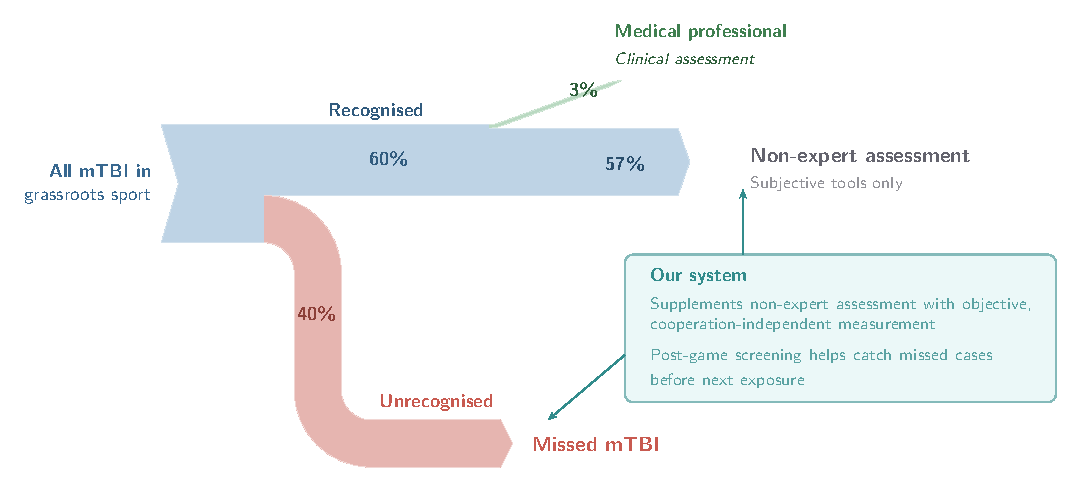
\includegraphics[width=\textwidth]{figures/intro_sankey.pdf}
    \caption{Estimated diagnostic pathway for mTBI in grassroots sport, showing where cases are currently missed. Proportions are approximate; see text for sources and discussion of evidence quality~\cite{mccrea2004unreported, echlin2010sideline, pryor2015athletic}.}
    \label{fig:intro_sankey}
\end{figure}

Mild traumatic brain injury (mTBI)\glsunset{mtbi}, commonly known as concussion, is the most prevalent form of neurological injury worldwide. An estimated 69 million people sustain traumatic brain injury annually~\cite{dewan2019estimating}, of which 70--90\% are classified as mild~\cite{cassidy2004incidence}. Critically, the majority of these injuries occur in community and youth sport settings where no medical professional is present to assess the injured individual.

In these settings, parents, teachers, coaches, and referees often act as de facto first responders yet lack access to objective screening tools. They must rely on visible signs and athlete self-reporting to decide whether medical evaluation is warranted. This approach is inadequate: approximately 50\% of concussions in youth and high school sports go unreported at the time of injury, with athletes failing to recognise the severity of their injury or being unwilling to remove themselves from competition~\cite{mccrea2004unreported, registermihalik2013knowledge}. Athletes routinely minimise symptoms to continue playing, and untrained observers cannot detect subtle neurological dysfunction without quantitative measurement.

The consequences of missed or delayed diagnosis are severe. Second impact syndrome, in which a second head injury is sustained before recovery from the first, causes catastrophic cerebral oedema and brain herniation and is frequently fatal~\cite{sis_statpearls}. Separately, post-concussive syndrome affects up to 15\% of adults following \ab{mtbi}~\cite{ppcs_statpearls}, with up to 50\% of patients symptomatic at three months and 27\% unable to return to their previous level of work at 12 months~\cite{mortaheb2021ppcs}. Early identification is therefore critical to enable appropriate management, prevent premature return to activity, and reduce the likelihood of long-term complications.

These findings establish a clear unmet need: an objective screening capability that can supplement existing non-expert assessment at the point of injury in grassroots sports settings. \Cref{fig:intro_sankey} illustrates this pathway and highlights where cases are currently missed. The 50\% unreporting rate is well-established~\cite{mccrea2004unreported}; bystander detection rates are inferred from video review and instrumented helmet studies~\cite{echlin2010sideline, beckwith2013impacts}, and medical coverage estimates from high school athletic trainer data~\cite{pryor2015athletic}.


\section{Limitations of Existing Approaches}
\label{chapter:introduction:limitations}

Current approaches to \ab{mtbi} assessment fall broadly into two categories: tools that are accessible in field settings but lack objective measurement, and tools that provide quantitative assessment but require clinical infrastructure. Neither addresses the need for objective, point-of-injury screening by non-medical personnel.

\textbf{Accessible but subjective.} The Concussion Recognition Tool 6 (CRT6) was designed specifically for use by non-medical personnel such as parents, coaches, and referees~\cite{echemendia2023crt6}. However, it provides only observational screening without quantitative metrics, requiring the observer to make subjective judgements about concerning signs. More broadly, all field-side assessment approaches that depend on patient self-reporting are vulnerable to symptom minimisation by athletes motivated to return to play. This is not limited to lay observers: athletes systematically underreport symptoms even when assessed by trained team medical personnel, with cleared athletes continuing to minimise symptoms days post-concussion~\cite{meier2015underreporting}. Tools accessible to non-experts thus depend on either patient cooperation or subjective clinical judgement, neither of which provides objective quantitative measurement.

\textbf{Objective but inaccessible.} The \ab{scat6} provides comprehensive evaluation combining symptom inventories, cognitive screening, neurological examination, and balance testing, but requires medical training for proper administration and interpretation~\cite{echemendia2023scat6}. Commercial quantitative pupillometry devices offer objective measurement but cost thousands of pounds and are designed for medical facilities rather than field deployment. The most recent American Congress of Rehabilitation Medicine diagnostic criteria explicitly acknowledge that no validated stand-alone objective diagnostic test is available, even to trained clinicians~\cite{silverberg2023acrm}. Alternative objective biomarkers face different but equally disqualifying limitations: blood biomarkers require venipuncture, laboratory processing, and hours to days of turnaround time, while neuroimaging modalities remain insensitive to the diffuse axonal injury that characterises \ab{mtbi} and require hospital facilities (detailed discussion in \Cref{chapter:background}).

In summary, accessible tools lack objectivity and depend on patient cooperation or subjective assessment, while objective tools require trained personnel, specialised equipment, or clinical infrastructure. No existing approach provides objective quantitative measurement that can supplement non-expert assessment at the point of injury.


\section{Project Objectives}

This project addresses the identified gap by developing a smartphone-based oculomotor assessment system designed to \textbf{supplement, not replace,} existing non-expert screening tools such as the CRT6 with objective, quantitative measurement. Rather, it strengthens the non-expert screening pathway by adding an automated, cooperation-independent measurement where currently only subjective observation is available.

The approach is motivated by evidence that oculomotor dysfunction is a commonly observed consequence of \ab{mtbi}, with the majority of affected individuals exhibiting abnormalities in eye movements and pupillary responses~\cite{mcdonald2022eye}. This prevalence reflects the vulnerability of distributed oculomotor control networks, spanning cortex, brainstem, and cerebellum, to the diffuse axonal injury that characterises \ab{mtbi} (detailed pathophysiology in \Cref{chapter:background}). Importantly, these responses are involuntary and cannot be consciously suppressed, making them robust to the patient cooperation problem identified in \Cref{chapter:introduction:limitations}.

The system implements three complementary oculomotor assessments: \ab{plr}, smooth pursuit eye movements, and vergence (\ab{npc}). Each provides independent diagnostic information, and multi-parameter assessment achieves superior performance compared to any single measure. Recent smartphone-based pupillometry research has demonstrated the technical feasibility of this approach, with published systems achieving diagnostic accuracy comparable to or exceeding conventional clinical tools~\cite{maxin2024smartphone}.

The system is designed to meet the following requirements:

\begin{itemize}
    \item \textbf{Accessible deployment:} Smartphone-based implementation using consumer device cameras eliminates the cost barrier of specialised equipment and enables deployment in any setting where smartphones are available.

    \item \textbf{Usability by non-experts:} Automated stimulus delivery and analysis eliminate the need for medical training or subjective interpretation.

    \item \textbf{Objective measurement:} Quantitative tracking of involuntary physiological responses provides assessment independent of patient self-reporting or cooperation.

    \item \textbf{High sensitivity:} The design prioritises detection of true \ab{mtbi} cases, accepting higher false positive rates as preferable to missed diagnoses in a screening context where positive results prompt medical referral rather than definitive diagnosis.

    \item \textbf{Rapid assessment:} Total assessment time targets under 10 minutes, enabling practical deployment during sports events, in school settings, or as routine post-game screening to help identify concussions not recognised during play.
\end{itemize}


\section{Scope and Ethical Considerations}

\textbf{Screening, not diagnosis.} The tool is designed as a screening instrument: it identifies individuals who may require further medical evaluation, but does not provide a clinical diagnosis of \ab{mtbi}. A positive result should prompt referral to a healthcare professional, not be treated as a definitive assessment.

\textbf{A negative result does not constitute clearance.} The system cannot reliably rule out concussion, and users must be made aware of this. The risk of over-reliance by non-expert users, who may interpret a negative screening result as permission to return to play, must be mitigated through clear communication in the application interface and accompanying guidance.

The system has not been validated on a clinical \ab{mtbi} population. The work presented in this report demonstrates technical feasibility and measurement accuracy on healthy participants, but establishing diagnostic sensitivity and specificity requires future clinical trials with confirmed concussion cases. This limitation is inherent to the project scope and timeline, and any claims regarding diagnostic performance are drawn from the existing literature rather than from our own clinical data.

Finally, the system collects oculomotor and biometric data, potentially from minors in sport settings. This carries data privacy obligations under UK GDPR, particularly regarding informed consent, data minimisation, and secure storage. The ethical implications of biometric data collection from vulnerable populations were considered throughout the design process, and all data collected during testing was handled in accordance with the University's ethical approval procedures. \todo{Detail specific data protection measures implemented (anonymisation, on-device processing, storage protocols).}
